\chapter{Electromagnetic forces}

\section{DC motor}
\begin{problem}
A current \(I\) is carried by a square coil of \(n\) turns
and side length \(L\). This coil is suspended vertically
in a uniform horizontal magnetic field of flux \(B\).
At time \(t\), the coil makes an angle \(\theta\) with
the vertical axis.

What is the torque experienced by the coil? Describe its motion.
\end{problem}

The vertical sides of the coil experience a magnetic force of magnitude
\(F = nBIL\). Since there are two opposite vertical sides in the coil,
the magnetic forces experienced by both sides form a \it{couple}.

Where \(d\) is the horizontal distance between the vertical sides,
\begin{align*}
	\tau & = Fd               \\
	     & = FL\cos\theta     \\
	     & = nBIL^2\cos\theta
\end{align*}

Since the coil never changes its shape, \(\tau = I_P\ddot{\theta}\),
where \(I_P = \f{1}{6}mL^2\) is the coil's moment of inertia, and \(\ddot{\theta}\) the angular acceleration.
We are left with a
second-order differential equation. This differential
equation unfortunately has no elementary solution.
\begin{equation*}
	\ddot{\theta} = \f{6nBI}{m} \cos\theta \propto \cos\theta
\end{equation*}

\section{Wire frame}
\begin{figure}[htpb]
	\centering
	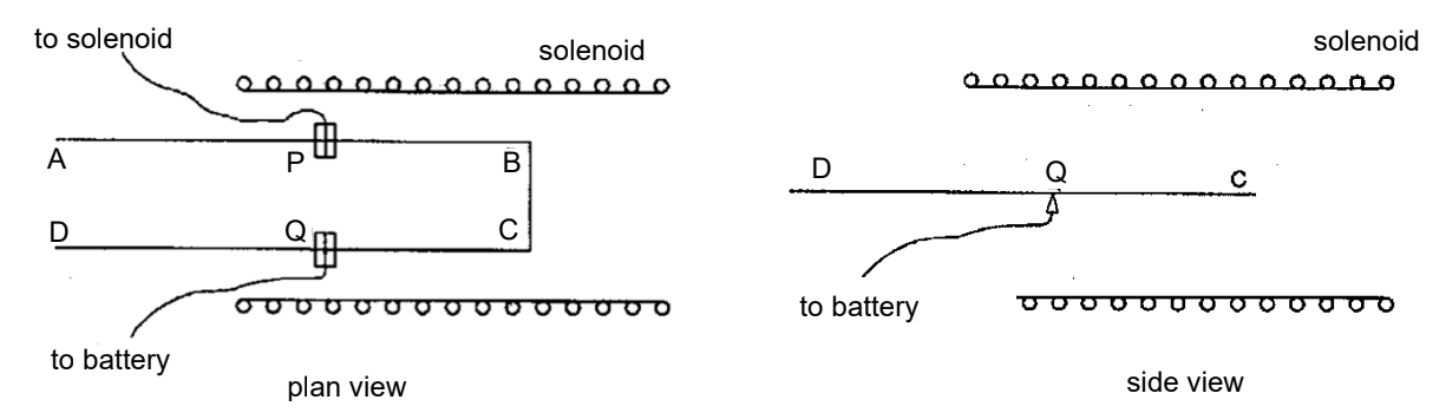
\includegraphics[scale=.5]{assets/wireframe.png}
	\caption{Wire frame}
	\label{fig:wireframe}
\end{figure}
\begin{problem}
A wire frame \(\text{ABCD}\) is supported in two knife-edges \(\text{P}\) and \(\text{Q}\)
so that \(\text{PBCQ}\) lies within a solenoid. Electrical connections are made to the frame
through the knife-edges, such that \(\text{PBCQ}\) may also be connected in series with
a battery. When there is no current in the circuit, the frame is horizontal.

In this configuration, what is the direction of the force due to the solenoid's magnetic field
acting on, respectively, side \(\text{BC}\) and side \(\text{PB}\)?
\end{problem}
\begin{itemize}
	\item Using the plan view, the current flows upwards from \(\text{C}\) to \(\text{B}\) and the magnetic
	      field is directed leftwards. Using \term{Fleming's Left-Hand Rule}, the magnetic force
	      on \(\text{BC}\) acts \hil{upwards}.
	\item On side \(\text{PB}\), the current is parallel to the magnetic field. This side experiences no magnetic force.
\end{itemize}

\begin{problem}
State two ways in which you could reverse the direction of the force on side \(\text{BC}\).
\end{problem}
\begin{enumerate}
	\item Swap the connections of the knife-edges \(\text{P}\) and \(\text{Q}\).
	\item Reverse the direction of the battery.
\end{enumerate}

\begin{problem}
The solenoid has \(n = \qty{700}{\per\metre}\) and carries a current \(I = \qty{3.5}{\ampere}\).
Calculate
\begin{enumerate}
	\item the magnetic flux density about side \(\text{BC}\);
	\item the force acting on side \(\text{BC}\) due to the magnetic field, given that its length \(l = \qty{5.0}{\centi\metre}\);
	\item the distance \(d\) from the knife-edge a mass of \(m = \qty{0.10}{\gram}\) must be placed on \(\text{DQ}\), such that the frame remains horizontal (\(\text{QC}\) is of length \(x = \qty{15.0}{\cm}\)).
\end{enumerate}
\end{problem}
\begin{enumerate}
	\item \(B = \mu_0nI = \hil{\qty{3.08e-3}{\tesla}}\)
	\item \(F = BIL = \hil{\qty{5.39e-4}{\newton}}\)
	\item Taking moments about the knife-edge \(\text{Q}\), \(Fx = mgd\). \(d = \lf{Fx}{mg} = \hil{\qty{8.24}{\cm}}\)
\end{enumerate}

\section{Ion source}
\begin{marginfigure}
	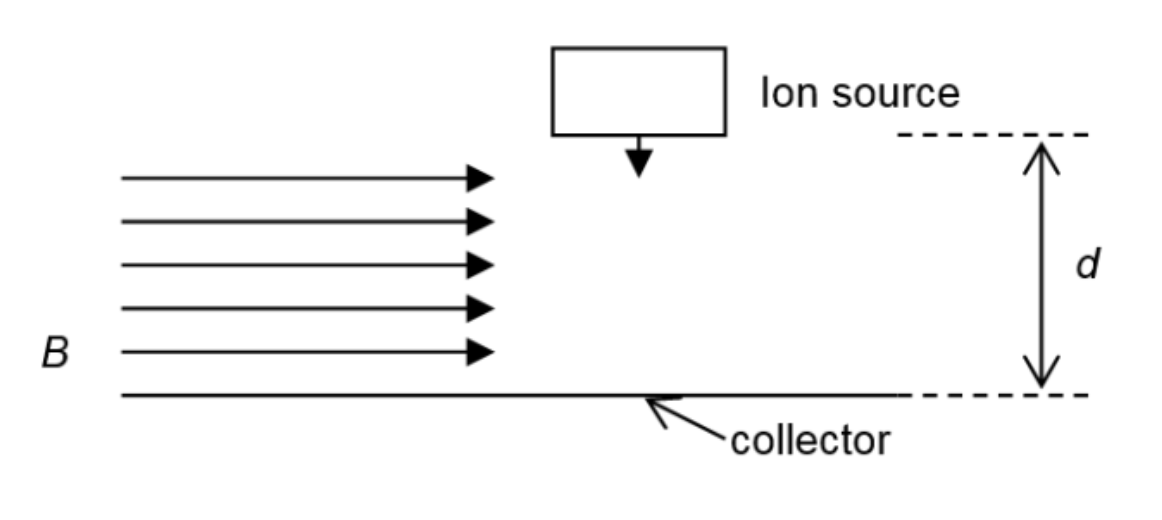
\includegraphics[scale=.25]{assets/ion-source.png}
	\caption{Ion source and collector}
	\label{fig:ionsource}
\end{marginfigure}
\begin{problem}
As in \cref{fig:ionsource}, an ion source is at a distance \(d\) from a flat, horizontal collector
at the same potential as the source. A uniform magnetic field of flux density \(B\) acts horizontally
in the region between the source and the collector.

An ion of charge \(q\) and mass \(m\) is emitted vertically downwards at speed \(v\). What
conditions does must \(v\) satisfy for the ion to reach the collector?
\end{problem}

When the ion enters the magnetic field, the magnetic force exerted on it
will cause the ion to undergo circular motion.
\begin{align*}
	Bqv & = \lf{mv^2}{r} \\
	r   & = \lf{mv}{Bq}
\end{align*}

The radius of the circular orbit must be sufficiently
large in order to leave the magnetic field, so \(r > d\).
Otherwise, the charge will continue orbiting within the magnetic field
and not reach the collector. \(\lf{mv}{Bq} > d\), thus \(v < \lf{Bdq}{m}\).

\section{Spiralling}
\begin{marginfigure}
	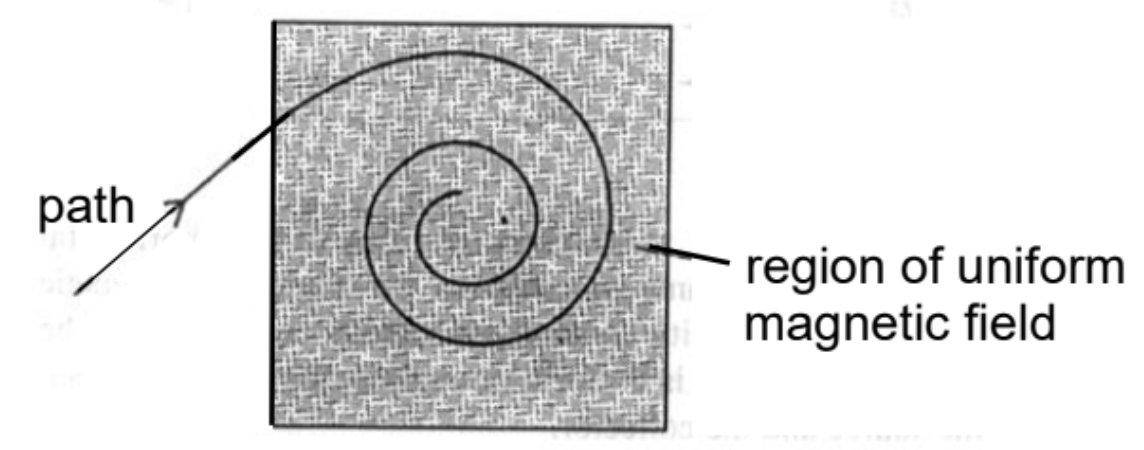
\includegraphics[scale=.25]{assets/spiralling-path.png}
	\caption{Spiralling path}
	\label{fig:spiralling}
\end{marginfigure}
\begin{problem}
A charged particle enters a uniform magnetic field at a right angle,
and traces the path in \cref{fig:spiralling}. Why?
\end{problem}

The magnetic force exerted on the charge provides the centripetal
force for its circular motion. \(Bqv = \lf{mv^2}{r}\), and so
\(r = \lf{mv}{Bq}\). As \(m\) and \(q\) are constants, there are two
plausible explanations:
\begin{itemize}
	\item \(v\) is decreasing---the particle must be losing energy;
	\item \(B\) is increasing---the magnetic flux the particle experiences must be increasing.
\end{itemize}
